% !TeX encoding = UTF-8
% !TeX spellcheck = de_DE
% !TeX program = pdflatex

% % % % % % % % %
% offene Punkte
% % % % % % % % %

%TODO „Konzentrationshilfe für eine längere Sitzung“ → auf den Leerseiten einfügen
%TODO Auzählungszeichen (z.B römisch 1) für Abschnitt „Infoblatt zum StartPaket“ vor dem 1. Kapitel

% % % % % % % % % % % % % % % % % %
% Dokumentation und Informationen
% % % % % % % % % % % % % % % % % %

% PDFs einbinden: keine technisch schöne Lösung, aber es geht schnell.
% Verbesserung für die Zukunft: Wiki-Seiten in geeignetem Format (z.B. DocBook-XML) exportieren (evtl. sogar automatisiert) und in LaTeX parsen.

% DRUCK
%  auf A4, mit Druckrändern von ca. 7mm an den kurzen und 6mm an den langen Kanten
%   (Die über die PDFs gelegten Seitennummern und Kapitelüberschriften sehr knapp an diesem Rand.)

% pdfbook --short-edge stuve-handbuch.pdf
% bzw.
% pdfjam --booklet 'true' --landscape --suffix book --signature '4' --preamble '\usepackage{everyshi}
% \makeatletter
% \EveryShipout{\ifodd\c@page\pdfpageattr{/Rotate 180}\fi}
% \makeatother
% ' -- stuve-handbuch.pdf - 







% Seitennummern in PDFs einfügen, Kapitelüberschriften Rand:
%  http://stackoverflow.com/questions/1603301/how-to-add-page-numbers-to-postscript-pdf
%  http://tex.stackexchange.com/questions/48641/chapter-title-in-rotated-vertical-box-at-the-margin

% Doku zum Einbinden von PDF-Seiten mit pdfpages:
%  http://www.ctan.org/tex-archive/macros/latex/contrib/pdfpages/pdfpages.pdf

% pdfpages verwendet letzendlich \includegraphics aus graphicx
%  ab Seite 9 aus http://ctan.mackichan.com/macros/latex/required/graphics/grfguide.pdf

% Altenative, ursprüngliche Realisierung mit pdfjam:
% pdfjam --outfile ./stuve-handbuch.pdf --fitpaper 'true' --twoside --paper a4paper --no-tidy --frame 'false' --rotateoversize 'false' --suffix joined -- 00-intro.pdf - 10-infoblatt-startpaket.pdf - aa-fuellseiten.pdf 1 20-grundsaetzliches-fsr.pdf - 40-aufgabenverteilung.pdf - 55-beschlusssammung-stex.pdf -  60-vs-dossier-rechtliche-rahmenbedingungen.pdf 1-17 aa-fuellseiten.pdf 2 70-organisationssatzung.pdf - 75-finanzordnung.pdf - 91-struktur	%fitpaper=true,-uebersicht.pdf - 92-struktur-akad_selbstverw.pdf - 93-struktur-besetzung-kontrolle.pdf - 99-extro.pdf -


\documentclass[
	8pt,
	a5paper,
	twoside
	]
	{book}

% !TeX root = ../stuve-handbuch-latex.tex
% !TeX encoding = UTF-8
% !TeX spellcheck = de_DE
% !TeX program = pdflatex



% Dokument-Metadaten:
% % % % % % % % % % %

\title{StuVe-Handbuch: Gremien, Beschl\"usse und Statuten}
\date{\today}
\author{et al.\email{stuve.kontakt@uni-ulm.de}}


% Schrifen, Sprache und Co.:
% % % % % % % % % % % % % % %

\usepackage[utf8]{inputenc}
\usepackage[T1]{fontenc}					% für echte Umlaute und mehr…
\usepackage{lmodern}						% schönere Schrift, v.a in PDFs
\renewcommand{\familydefault}{\sfdefault}
\usepackage[ngerman]{babel}					% deutsche Sprachvariante (Inhaltsverzeichnis, …)
\usepackage{setspace}
\usepackage{tipa}							% für IPA Zeichen


% Textbild:
% % % % % %

\setlength{\parindent}{0pt}        %  kein Einruecken bei Absaetzen 


% „Seiteneinstellungen“:
% % % % % % % % % % % %

% Fußnoten:
\usepackage{perpage}
\MakePerPage{footnote}		%perpage package command: fußnoten

\usepackage[left=2.2cm, right=2cm, top=1cm, bottom=1cm]{geometry}
% Diese „Seitengeometrie“ passt ganz gut zu einem Heftchen aus DIN A5 Seiten mit einer Ringbindung (Plastik), wie man sie im Druckraum der StuVe herstellen kann.
% Abschätzung / Uberlegungen:
%  * Die Rinbindung wird bei 38 Blatt DIN A5 (76 Seiten mi PDF) mit 80 g/m² mit einem 10 mm Binderücken aus Plastik ganz gut.
%  * Die Löcher für die Ringbindung nehmen ca. 7 mm vom inneren Papierrand in der Breite weg.
%  * Am äußeren Rand der Seiten nehmen dir überlagerten Seitennummern und die denkrechten Abschnittsüberschriften optisch noch Platz ein. Die entsprechenden Maße finden sich unten (Definition des eigenen 'fancypagestyle'),
%  * Eigentlich ist's so gedacht, dass das Heft ohne nachträgliche Skalierung auf dem Weg zum Drucker gedruckt wird, jedoch passiert das je nach Drucker und Druckertreiber evtl. trotzdem.



\usepackage{layout}							% für \layout{} → Darstellung der aktuellen Ränder und Co.
\usepackage{totcount}						% Zählen der Gesamtzahl, z.B. von Kapiteln
\regtotcounter{chapter}

\usepackage[final]{pdfpages}
\usepackage{graphicx}


% Überschriften und Inhaltsverzeichnis formatieren:
% % % % % % % % % % % % % % % % % % % % % % % % % %

\addto\captionsngerman{\renewcommand{\chaptername}{Teil}}

\usepackage{titlesec}
\usepackage{fancyhdr}

\renewcommand*{\chaptermark}[1]{ \markboth{\thechapter: ##1}{} }%

%\titlespacing*{\chapter}{0pt}{}{20pt}
\titleformat{\chapter}[display]{\normalfont\huge\bfseries}{\flushright \chaptertitlename\ \thechapter}{5pt}{\flushright \Huge}

% Neues Kommando zum individuellen Einfügen des Inahltsverzeichnisses:
\makeatletter
\newcommand*{\toccontents}{\@starttoc{toc}}
\makeatother

\usepackage{titletoc}

% Merkhilfe:
% \titlecontents{⟨Abschnitt⟩}[⟨Links⟩]{⟨Gesamtformatierung⟩}{⟨Vor dem Label⟩}{⟨Nach dem Label⟩}{⟨Abstandsfüller & Seitenzahl⟩}[⟨Rechts⟩]
\titlecontents{chapter}[1.5em]{\small}{\contentslabel{1em}}{}{\titlerule*[0.3pc]{.}\contentspage}
\titlecontents{section}[2.5em]{\footnotesize}{\contentslabel{1em}}{}{\titlerule*[0.3pc].{}\contentspage}
%\titlecontents{subsection}[6.7em]{}{\contentslabel{2.95em}}{}{\titlerule*[0.3pc]{.}\contentspage} 
%\titlecontents{subsubsection}[10.6em]{}{\contentslabel{3.8em}}{}{\titlerule*[0.3pc]{.}\contentspage}
%\titlecontents{paragraph}[15.25em]{}{\contentslabel{4.6em}}{}{\titlerule*[0.3pc]{.}\contentspage}


% Abschnittsmarkierungen (äußerer Seitenrand)
% % % % % % % % % % % % % % % % % % % % % % %

\usepackage{tikz}
\usepackage{color}
\usetikzlibrary{shapes.misc}
\usetikzlibrary{calc}
\usetikzlibrary{positioning}
\usepackage{lipsum}

\usepackage{etoolbox}
% Patch the sectioning commands to provide a hook to be used later
\preto{\chapter}{\def\leveltitle{\chaptertitle}}
\preto{\section}{\def\leveltitle{\sectiontitle}}
\preto{\subsection}{\def\leveltitle{\subsectiontitle}}
\preto{\subsubsection}{\def\leveltitle{\subsubsectiontitle}}

\makeatletter
% \@sect is called with normal sectioning commands
% Argument #8 to \@sect is the title
% Thus \section{Title} will do \gdef\sectiontitle{Title}
\pretocmd{\@sect}
{\expandafter\gdef\leveltitle{#8}}
{}{}
% \@ssect is called with *-sectioning commands
% Argument #5 to \@ssect is the title
\pretocmd{\@ssect}
{\expandafter\gdef\leveltitle{#5}}
{}{}
% \@chapter is called by \chapter (without *)
% Argument #2 to \@chapter is the title
\pretocmd{\@chapter}
{\expandafter\gdef\leveltitle{#2}}
{}{}
% \@schapter is called with \chapter*
% Argument #1 to \@schapter is the title
\pretocmd{\@schapter}
{\expandafter\gdef\leveltitle{#1}}
{}{}
\makeatother

%\newcommand\MyColor{
%	\ifcase\thechapter blue!30\or red!30\or olive!30\or magenta!30\else yellow!30\fi} 
\newcommand\MyColor{ black!30 }

\fancypagestyle{plain}{%
	%% Clear all headers and footers
	\fancyhf{}
	%% Right headers on odd pages
	\fancyhead[RO]{%
			\begin{tikzpicture}[overlay,remember picture]
			\ifdefined\chaptertitle
			\node[
				fill=\MyColor, text=black,
				font=\footnotesize,
				inner ysep=4pt, inner xsep=4pt,
				rounded rectangle,
				anchor = west,
				%xshift=-0mm,
				%yshift=-0mm,
				%text width=3cm,
				text height=0.3cm,
				rotate=90
			]
			% 21 cm an der kurzen Kante der A4 bzw. langen Kante der A5 Seite:
			%   21 cm - 6 mm Druckrand oben - 6 mm Druckrand unten - 6 mm Länge Bobbel Seitenzahl = 19,2 cm
			at ($ (current page.north east) + (-0.9cm, -0.7cm) + (-0.15cm, -0.3cm) + (0cm, -19.3 / \totvalue{chapter} * \thechapter cm) $)
			{\sffamily\normalsize\nouppercase{\thechapter: \chaptertitle}};
%			{\sffamily\normalsize\nouppercase{\thechapter: }};
			\fi
			\node[
				fill=\MyColor,text=black,
				font=\footnotesize,
				inner ysep=4pt, inner xsep=4pt,
				rounded rectangle,
				%anchor = north east,
				%xshift=-0mm,
				%yshift=-0mm,
				%text width=5cm,
				text height=0.3cm,
				rotate=0
			]
			at ($ (current page.north east) + (-0.9cm, -0.7cm) + (-0.15cm, -0.15cm) $)
			{\sffamily\normalsize\nouppercase{\thepage}};
			\end{tikzpicture}
	}
	%% Left headers on even pages
	\fancyhead[LE]{%
			\begin{tikzpicture}[overlay,remember picture]
			\ifdefined\chaptertitle
			\node[
			fill=\MyColor,text=black,
			font=\footnotesize,
			inner ysep=4pt, inner xsep=4pt,
			rounded rectangle,
			anchor=east,
			%xshift=-0mm,
			%yshift=-0mm,
			%text width=3cm,
			text height=0.3cm,
			rotate=270
			]
			at ($ (current page.north west) + (0.9cm, -0.7cm) + (0.15cm, -0.3cm) + (0cm, -19.3 / \totvalue{chapter} * \thechapter cm) $)
			{\sffamily\normalsize\nouppercase{\thechapter: \chaptertitle}};
%			{\sffamily\normalsize\nouppercase{\thechapter:}};
			\fi
			\node[
			fill=\MyColor,text=black,
			font=\footnotesize,
			inner ysep=4pt, inner xsep=4pt,
			rounded rectangle,
			%anchor= ,
			%xshift=-0mm,
			%yshift=-0mm,
			%text width=5cm,
			text height=0.3cm,
			rotate=0
			]
			at ($ (current page.north west) + (0.9cm, -0.7cm) + (0.15cm, -0.15cm) $)
			{\sffamily\normalsize\nouppercase{\thepage} };
			\end{tikzpicture}
	}
	\renewcommand{\headrulewidth}{0pt}
	\renewcommand{\footrulewidth}{0pt}
	%\fancyfoot[R]{\thepage}
}
% ----------------------------------------------------------------



% Hyperref-Paket (muss immer als letztes geladen werden)
% % % % % % % % % % % % % % % % % % % % % % % % % % % % %

\usepackage{hyperref}

\hypersetup{
	pdftitle=StuVe-Handbuch,
	pdfauthor=et. al.,
	pdfsubject={Handbuch},
	pdfproducer={pdflatex},
	%	colorlinks=false,
	pdfborder=0 0 0	% keine Box um die Links!
}


% Eigene Kommandos:
% % % % % % % % % %

% Führende Null für's Datum:
\newcommand{\leadingzero}[1]{\ifnum #1<10 0\the#1\else\the#1\fi} 

\begin{document}

%\layout{}

\frontmatter

\pagestyle{empty}

% !TeX root = ../stuve-handbuch-latex.tex
% !TeX encoding = UTF-8
% !TeX spellcheck = de_DE
% !TeX program = pdflatex

{
\newgeometry{left=2.7cm, right=2cm, top=1cm, bottom=1cm}
\pagestyle{empty}

%----------------------------------------------------------------------
%
%        Titelblatt
%
%----------------------------------------------------------------------

\begin{titlepage}

\null
\vfill

\begin{center}
	\vspace{2em}
	{\Huge \bfseries StuVe-Handbuch\\}
	\vspace{4em}
\end{center}

\begin{figure}[tbph]
\centering

\includegraphics[trim = 600px 0 600px 0, width = \linewidth]{./grafiken/VS_Scrabble-mod.jpg}
\end{figure}

\null
\vfill

\begin{center}
	\begin{minipage}{\textwidth}
	\begin{minipage}[b][2cm]{0.79\textwidth}
		\begin{flushleft}
			Version \the\year"~\leadingzero{\month}"~\leadingzero{\day}\\
			\vspace{0.5\baselineskip}
			StuVe / Verfasste Studierendenschaft\\
			Universität Ulm
		\end{flushleft}
	\end{minipage}
	\begin{minipage}[b][2cm]{0.2\textwidth}
		\begin{flushright}
			
\includegraphics[height=1.6cm]{./grafiken/stuve_logo_gedreht-leicht_grau.png}
		\end{flushright}
	\end{minipage}
\end{minipage}
\end{center}

\end{titlepage}

%\restoregeometry
%}

%----------------------------------------------------------------------
%
%        Innenseite
%
%----------------------------------------------------------------------
%{
%\newgeometry{left=2.7cm, right=2cm, top=1cm, bottom=1cm}

\newpage
\footnotesize
\bigskip


\begin{center}

\null
\vspace{2em}
\textbf{Wichtige Adressen}

\bigskip
Homepage\\
\textit{http://www.uni-ulm.de/stuve}

\bigskip
Wiki\\
\textit{https://wiki.asta.uni-ulm.de}

\bigskip
E-Mail\\
\textit{stuve@uni-ulm.de\\
stuve.exekutive@uni-ulm.de\\
stuve.kontakt@uni-ulm.de}\\

\null
\begin{minipage}{0.5\textwidth}
	\scriptsize
	\begin{center}
	Für Organisatorisches oder falls es wichtige Gründe gibt die StuVe-Liste nicht zu nutzen gibt es für StuPa und FSR eigene Listen. \\\textbf{Grundsätzlich soll jedoch stuve@uni-ulm.de genutzt werden!}
	\end{center}
\end{minipage}

\null
\textit{stuve.parlament@uni-ulm.de\\
stuve.fachschaftenrat@uni-ulm.de}

\bigskip
Mailinglisten\\
{\scriptsize (An- und Abmelden, Empfangsmodus, ...)}\\
\textit{https://imap.uni-ulm.de/lists}

\null
\vfill
\begin{minipage}{0.8\textwidth}
\footnotesize Dieses Heft gehört:~\hrulefill~;-)
\end{minipage}
\vspace{2em}
\null

\end{center}

\restoregeometry
}

% !TeX root = ../stuve-handbuch-latex.tex
% !TeX encoding = UTF-8
% !TeX spellcheck = de_DE
% !TeX program = pdflatex


\textit{Definition: Die Verfasste Studierendenschaft der Universität Ulm (VS) setzt sich aus allen eingeschriebenen Studierenden zusammen.
Die VS bzw. die Studierenden organisieren sich in der StuVe (StudierendenVertretung)\footnote{\today: Diese Definition der StuVe fehlt noch in der Organisationssatzung, sollte demnächst ergänzt werden.}.
D.h.\ alle Organe, Strukturen und auch sonst irgendwie offiziell aktiven Studierenden bilden die „organisierte“ StuVe – im Ggs. zur gesamten Studierendenschaft.}


\section*{Zu diesem Heft}

%\vspace{1em}
%\textbf{Zu diesem Handbuch}
%\vspace{0.3em}

Für alle in der StuVe Aktiven und insbesondere die Mitglieder der StuVe-Gremien sind die hier die wichtigsten Texte zusammengefasst, die die Grundlage für die Organisation und Arbeit der StuVe bilden. Ergänzend zu diesem Handbuch soll demnächst noch ein zweites Handbuch mit Hilfen für's operative Tagesgeschäft verfügbar sein.
Es handelt sich hier nicht um ein am Stück geschriebenes Werk, sondern fast ausschließlich um eine Zusammenstellung verschiedener Texte.
Einerseits sind einfache Hilfestellungen, wie z.B.\ die Infoblätter oder Grafiken, andererseits aber auch für alle Studierenden und insbesondere die gewählten Vertreter und Aktiven rechtlich verbindliche Texte, wie z.B.\ die Organisationssatzung oder die Finanzordnung, enthalten.

Da sich die Dokumente bisweilen ändern wird auch dieses Heft immer wieder aktualisiert werden, zum Vergleich verschiedener Ausgaben dient das Datum auf der Titelseite.
Manche der enthaltenen Dokumente haben eine eigene Seitennummerierung – im gesamten Heft ist jedoch jeweils am äußeren Rand die Bezeichnungen des aktuellen Teils und eine durchgehende Seitennummern grau hinterlegt abgedruckt. Auf diese bezieht sich das folgende Inhaltsverzeichnis.


\subsection*{Inhalt}

%\vspace{1em}
%\textbf{Inhalt}
%\vspace{0.3em}

\toccontents


\subsubsection*{Nicht enthalten}
%\vspace{0.5em}
%\textbf{Nicht enthalten}
%\vspace{0.3em}
\begin{itemize}
	\item Wahlordnung
	\item Landeshoschulgesetz Baden-Württemberg (LHG)\\Informationen hierzu jedoch in Rechtliche Grundlagen und Rahmenbedingungen für die neue Studierendenvertretung.
\end{itemize}



% % % % % % % % % % % % %
%
% AB HIER PDFs EINBINDEN
%
% % % % % % % % % % % % %


% Optionen für alle einzubindenden PDFs
\includepdfset{
	pages= - ,								% standardmäßig alle Seiten eines PDFs einbinden
	pagecommand=\thispagestyle{plain},
	%openright,								% lieber lassen :P
	%frame=true,							% für den Entwurfsmodus, vor dem Druck deaktivieren
	offset = 0.2cm 0,						% Zugabe für's Binden !!! weitere offsets unten sind zusätzlich
	trim = 1cm 0cm 1cm 0cm,
}

% die einzelnen PDFs beschneiden:
%	trim = l u r o
%		→ links, unten, rechts, oben etwas abschneiden, muss leider pro PDF definiert werden.

% beschnittene PDFs werden mit dem folgenden pauschal skaliert, so dass sie die Seite gut Ausnutzen
% nur eine Dimension (height) angegeben -> für PDFs gilt keepaspectratio, bei Grafiken einzeln drauf achten
\let\ORIincludegraphics\includegraphics
\renewcommand{\includegraphics}[2][]{\ORIincludegraphics[height=0.90\paperheight,#1]{#2}}



%\chapter{Infoblatt zum StartPaket}\newline\null
\addcontentsline{toc}{chapter}{StartPaket: Infoblatt\newline{\scriptsize\textit{\null\hspace{2em}Anleitung zum Kennenlernen wichtiger Einrichtungen und Arbeitsmaterialien}}}
%{\tiny\textit{Anleitung zum Kennenlernen wichtiger Einrichtungen und Arbeitsmaterialien}}
\clearpage
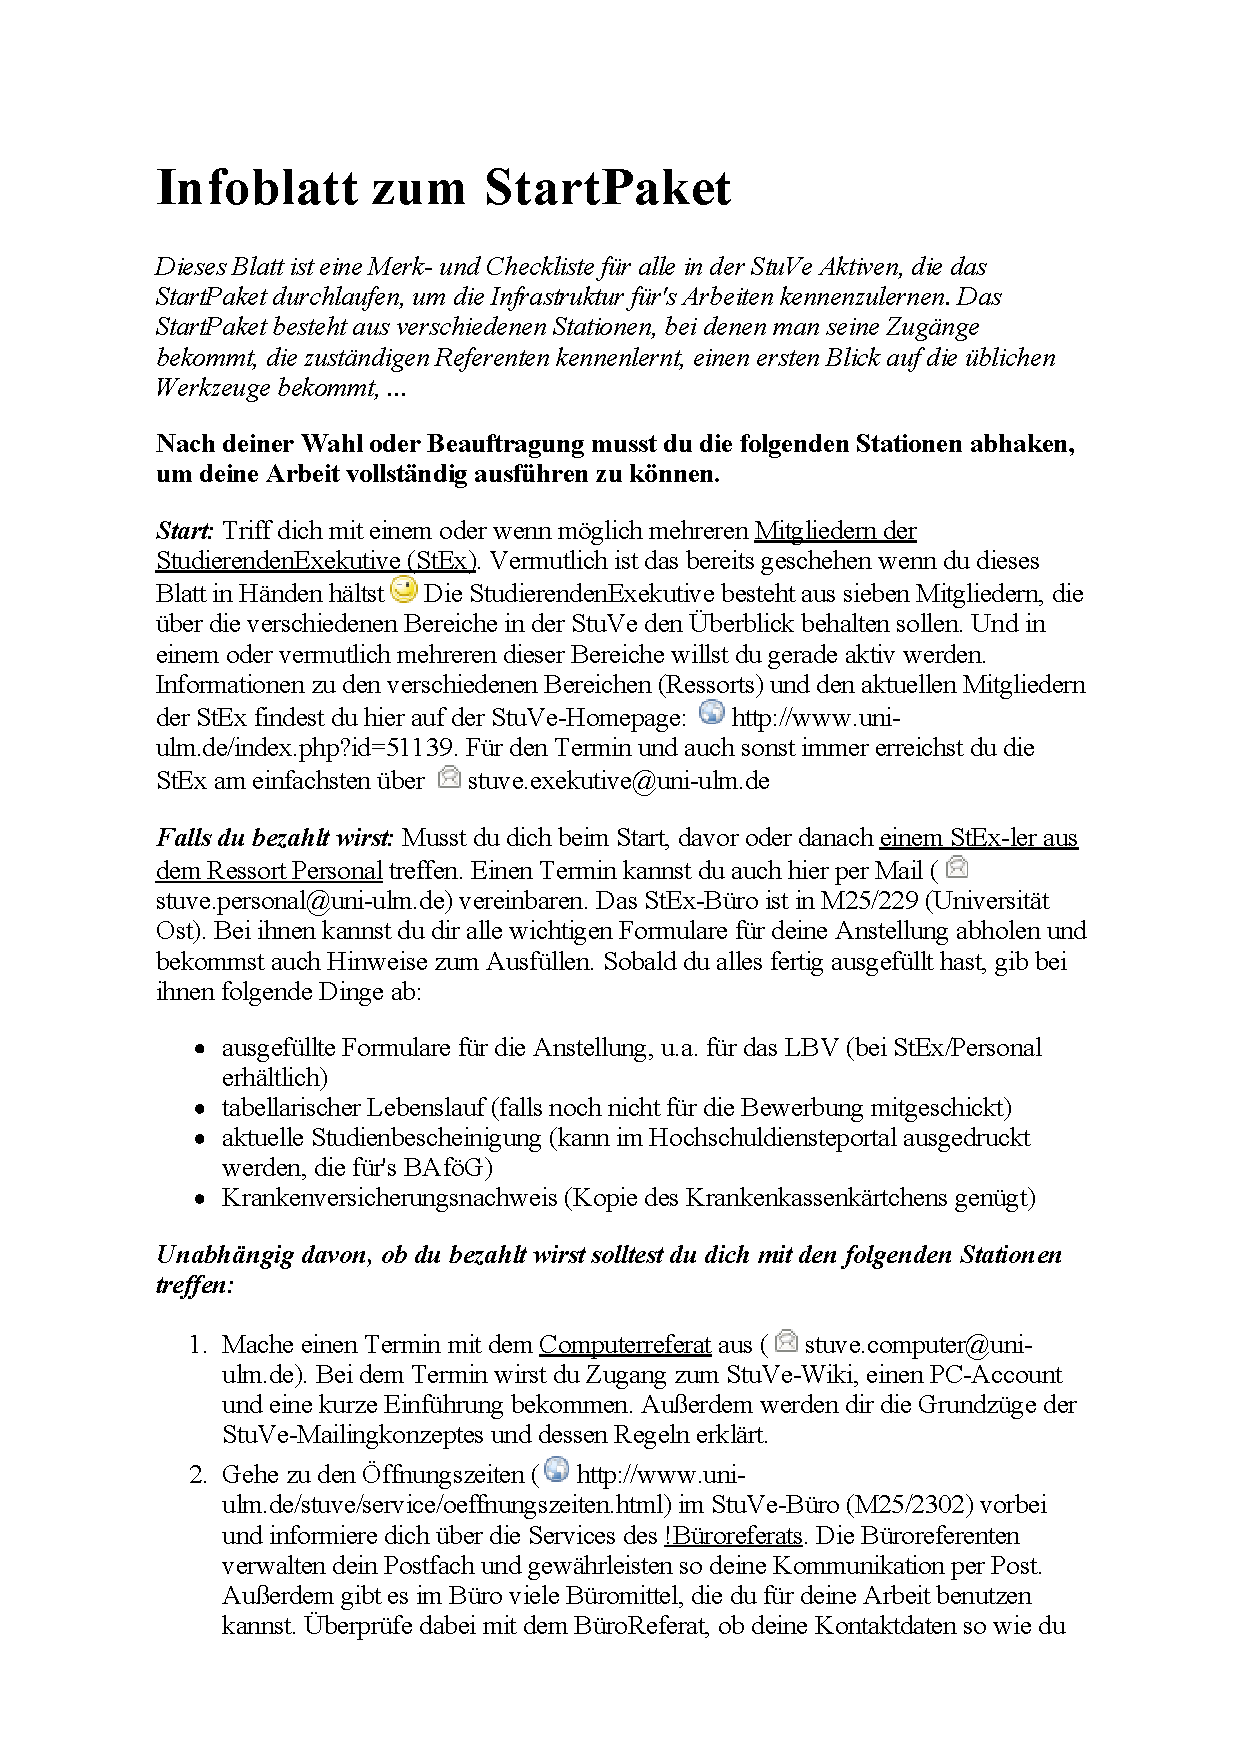
\includepdf
	[
		trim = 2cm 1.3cm 2cm 0.8cm,
		pagecommand=\thispagestyle{empty}
	]
	{./teile/10-infoblatt-startpaket.pdf}



\mainmatter

\pagestyle{plain}

\chapter{Gremienarbeit}
%\addcontentsline{toc}{chapter}{Gremienarbeit}

\clearpage

\addcontentsline{toc}{section}{Grundsätzliches für die Arbeit im FSR\newline{\scriptsize\textit{\null\hspace{2em}für die Arbeit im FSR bewährte “best practices”}}}

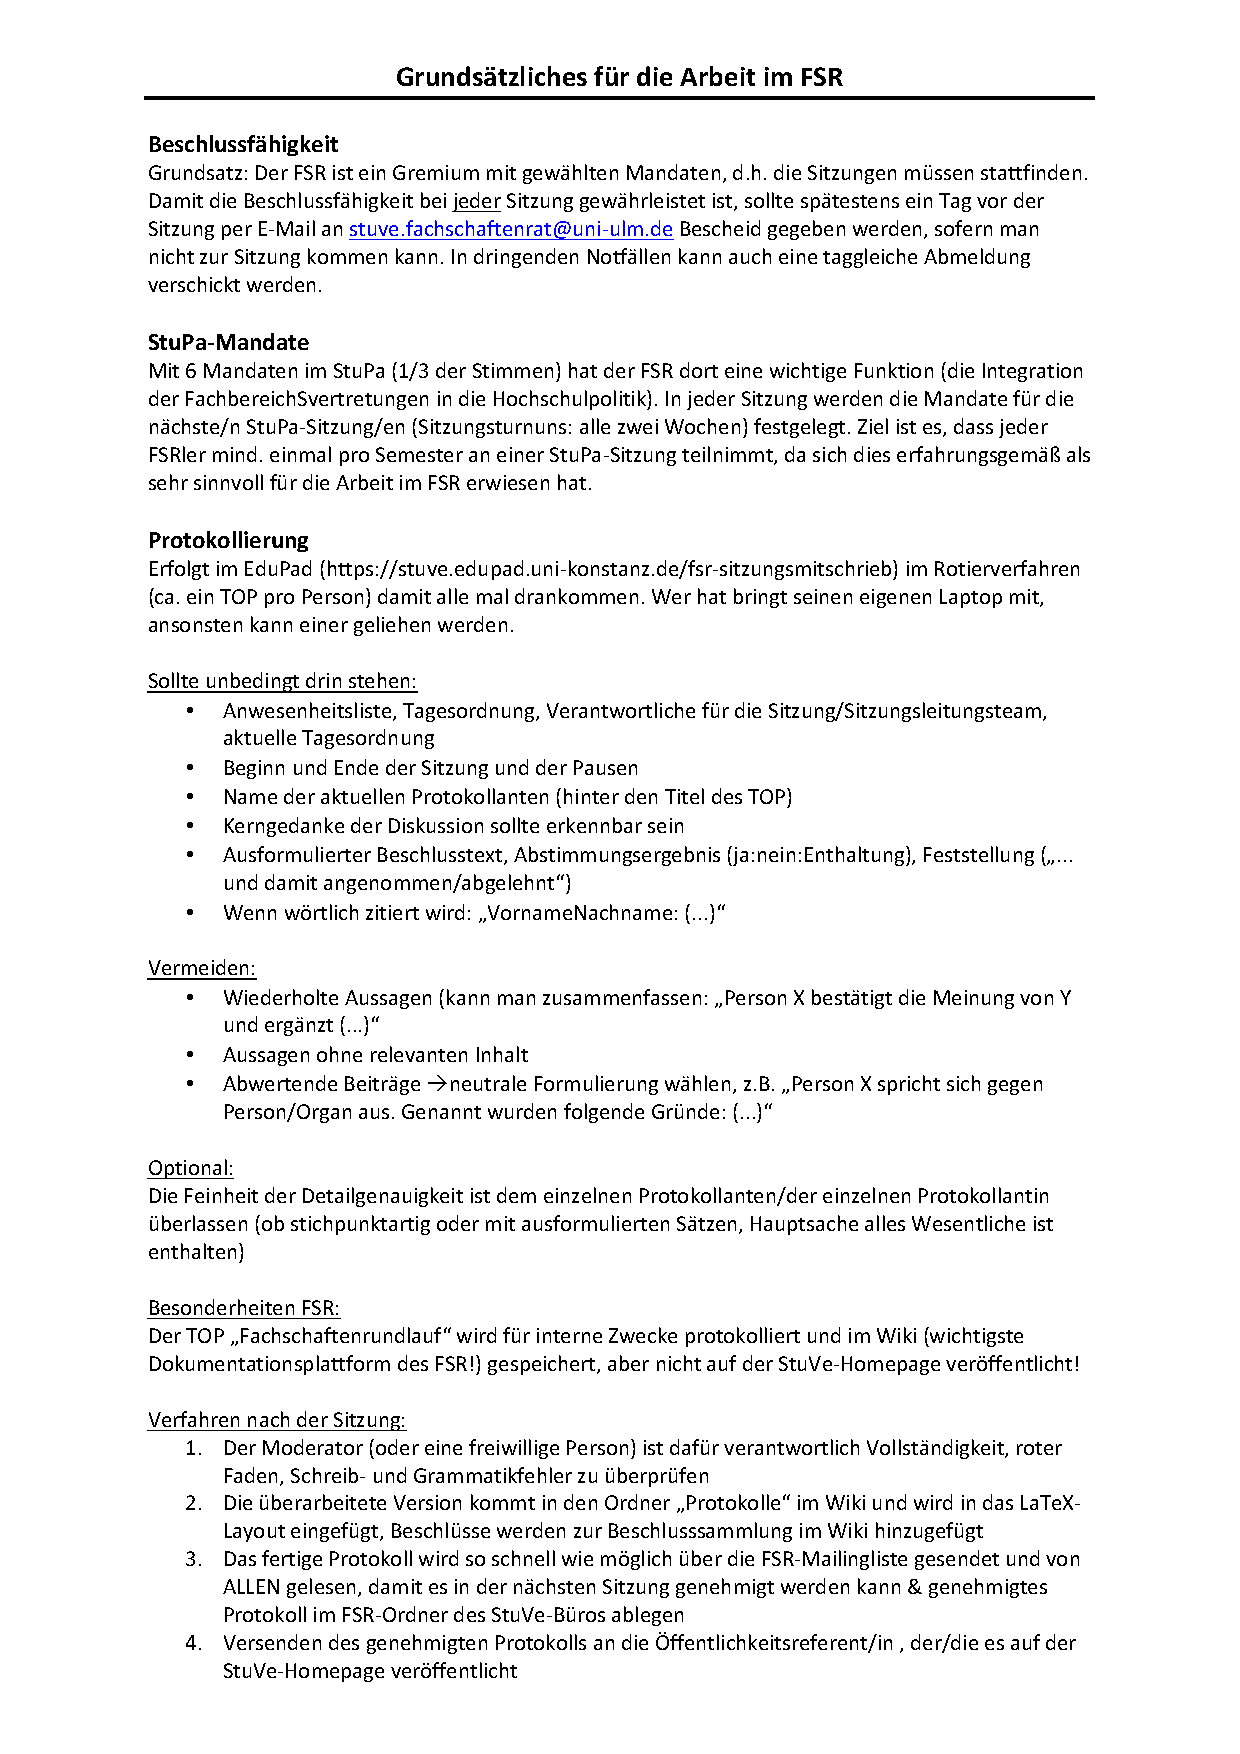
\includepdf
	[
		trim = 2cm 1cm 2cm 1cm,
		height = 0.95\paperheight,
		offset = -0.2cm 0cm
	]
	{./teile/20-grundsaetzliches-fsr.pdf}

\addcontentsline{toc}{section}{Grundsätzliches für die Arbeit im StuPa\newline{\scriptsize\textit{\null\hspace{2em}für die Arbeit im StuPa bewährte “best practices”}}}


\addcontentsline{toc}{section}{Aufgabenverteilung zwischen StuPa und FSR}

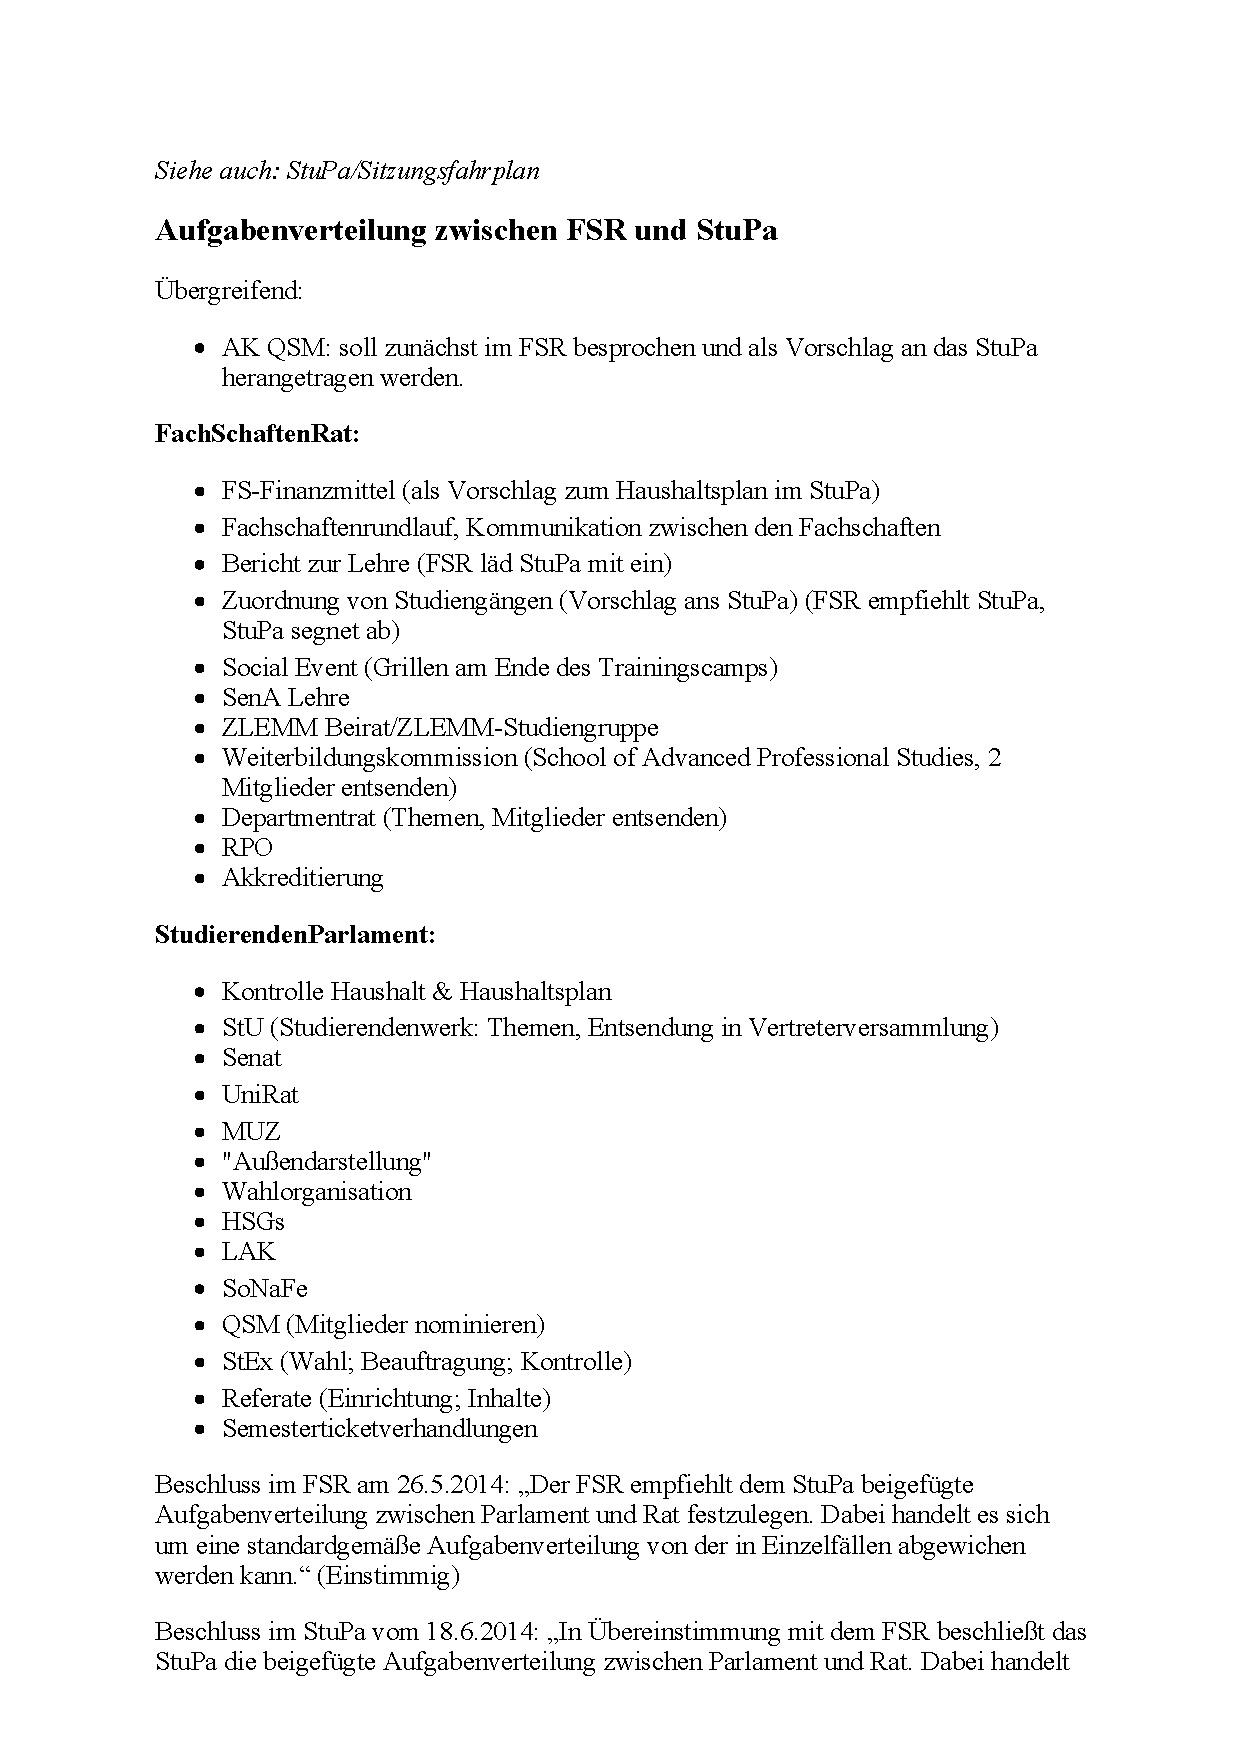
\includepdf
	[
		trim = 2cm 1.3cm 2cm 0.8cm
	]
	{./teile/40-aufgabenverteilung.pdf}


\chapter{Beschlusssammlungen}


\clearpage

%\addcontentsline{toc}{chapter}{Beschlusssammlungen}

%\addcontentsline{toc}{chapter}{Beschlüsse des StuPa}
%
%\addcontentsline{toc}{chapter}{Beschlüsse des FSR}
%
%\addcontentsline{toc}{chapter}{Beschlüsse der StEx}


\includepdf
	[
		trim = 2cm 1.3cm 2cm 0.8cm
	]
	{./teile/51-beschlusssammlung-stupa.pdf}


\includepdf
	[
		trim = 2cm 1.3cm 2cm 0.8cm
	]
	{./teile/55-beschlusssammung-stex.pdf}


\chapter{Rechtliche Grundlagen}

\textit{Stand 27.11.2013, d.h. Änderungen der LHG-Novelle vom April 2014 nicht enthalten. Dieser Teil wird evtl. erst nach Lesen der Organisationssatzung klar, kann aber auch vorab schon den „großen Rahmen“ erläutern.}

\clearpage

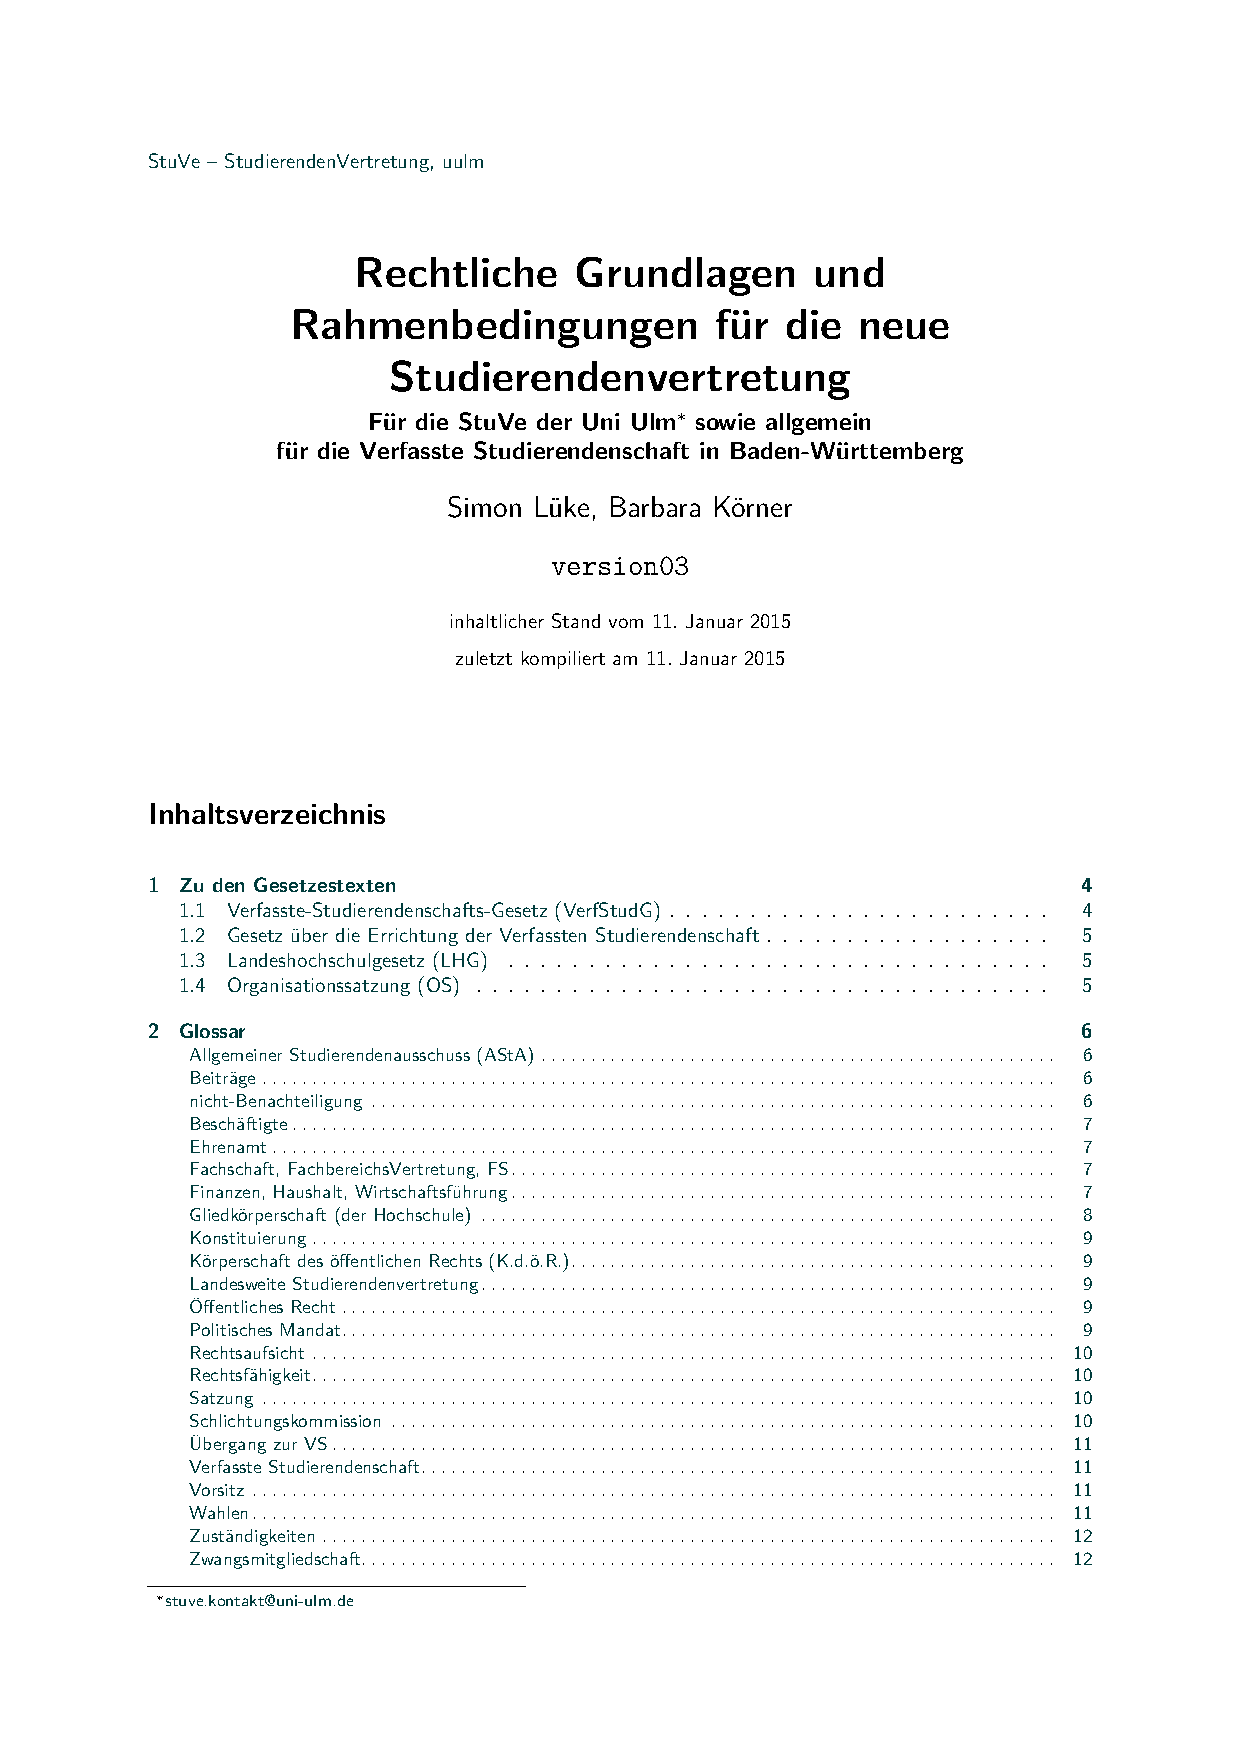
\includepdf
	[
		pages = 1-17,
		trim = 2cm 2cm 2cm 1cm
	]
	{./teile/60-vs-dossier-rechtliche-rahmenbedingungen.pdf}


\chapter{Organisationssatzung}

\textit{Obacht: Anhang A der Organisationssatzung ist nicht mehr aktuell. Masterstudiengang Software Engineering (neu) und Masterstudiengang Cognitive Systems (neu) sind der FS Informatik zugeordnet; Masterstudiengang Energy Science and Technology (bisher FS Elektrotechnik) ist der FS Chemie zugeordnet.}

\clearpage


\includepdf
	[
		trim = 2cm 2cm 2cm 1cm
	]
	{./teile/70-organisationssatzung.pdf}


\chapter{Beitragsordnung, Finanzordnung}


\clearpage


\includepdf
[
trim = 2cm 2cm 2cm 1cm
]
{./teile/74-beitragsordnung.pdf}


\includepdf
	[
		trim = 2cm 2cm 2cm 1cm
	]
	{./teile/75-finanzordnung.pdf}


\chapter{Grafiken}

\clearpage

\addcontentsline{toc}{section}{Übersicht}

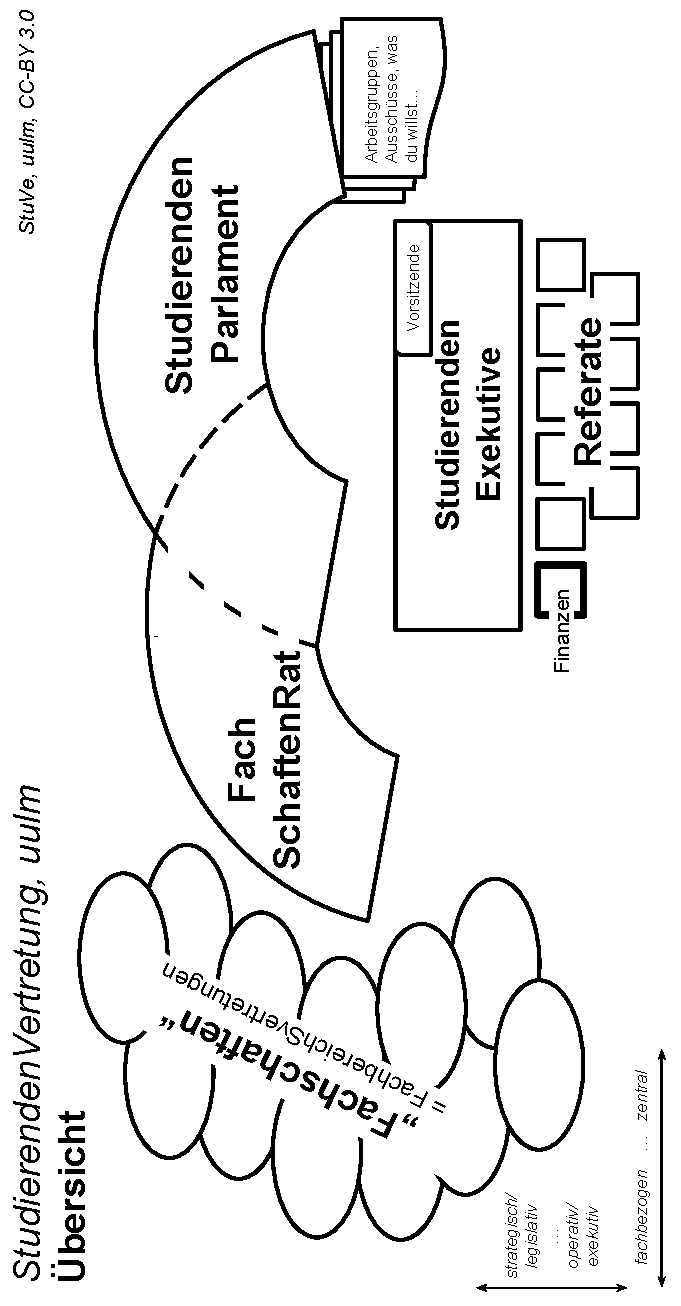
\includepdf
	[
		height = 0.9\paperheight,
		width = 0.8\paperwidth,
		keepaspectratio
	]
	{./teile/91-struktur-uebersicht.pdf}


\addcontentsline{toc}{section}{Studentische und akademische Selbstverwaltung}

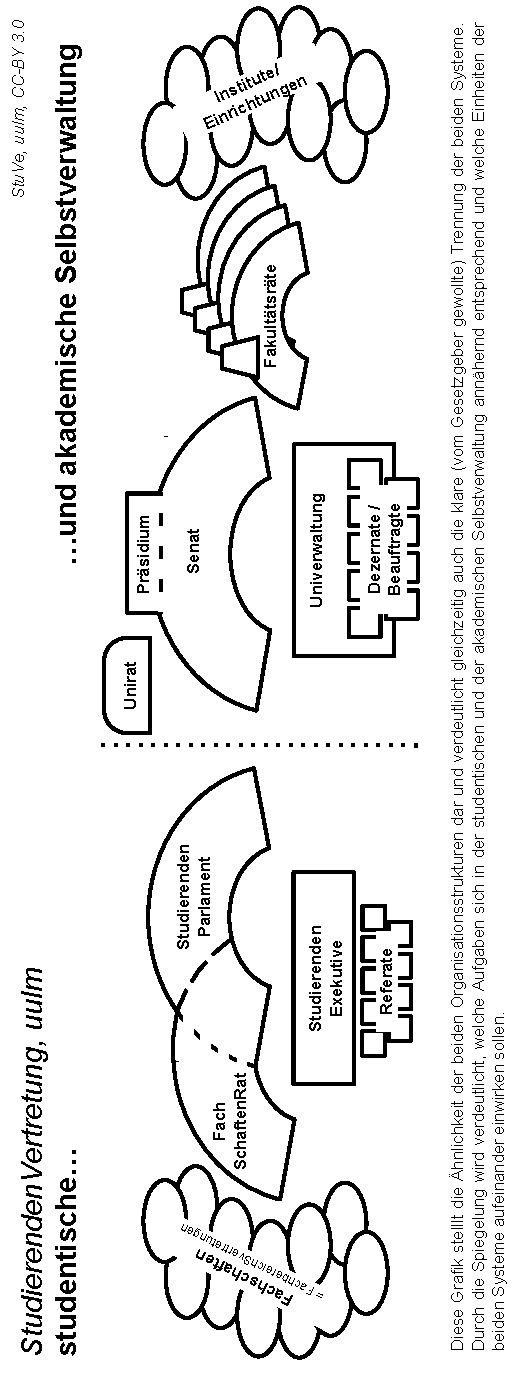
\includepdf
	[
		height = 0.9\paperheight,
		width = 0.8\paperwidth,
		keepaspectratio
	]
	{./teile/92-struktur-akad_selbstverw.pdf}


\addcontentsline{toc}{section}{Details: Besetzung, Interaktion und Kontrolle}

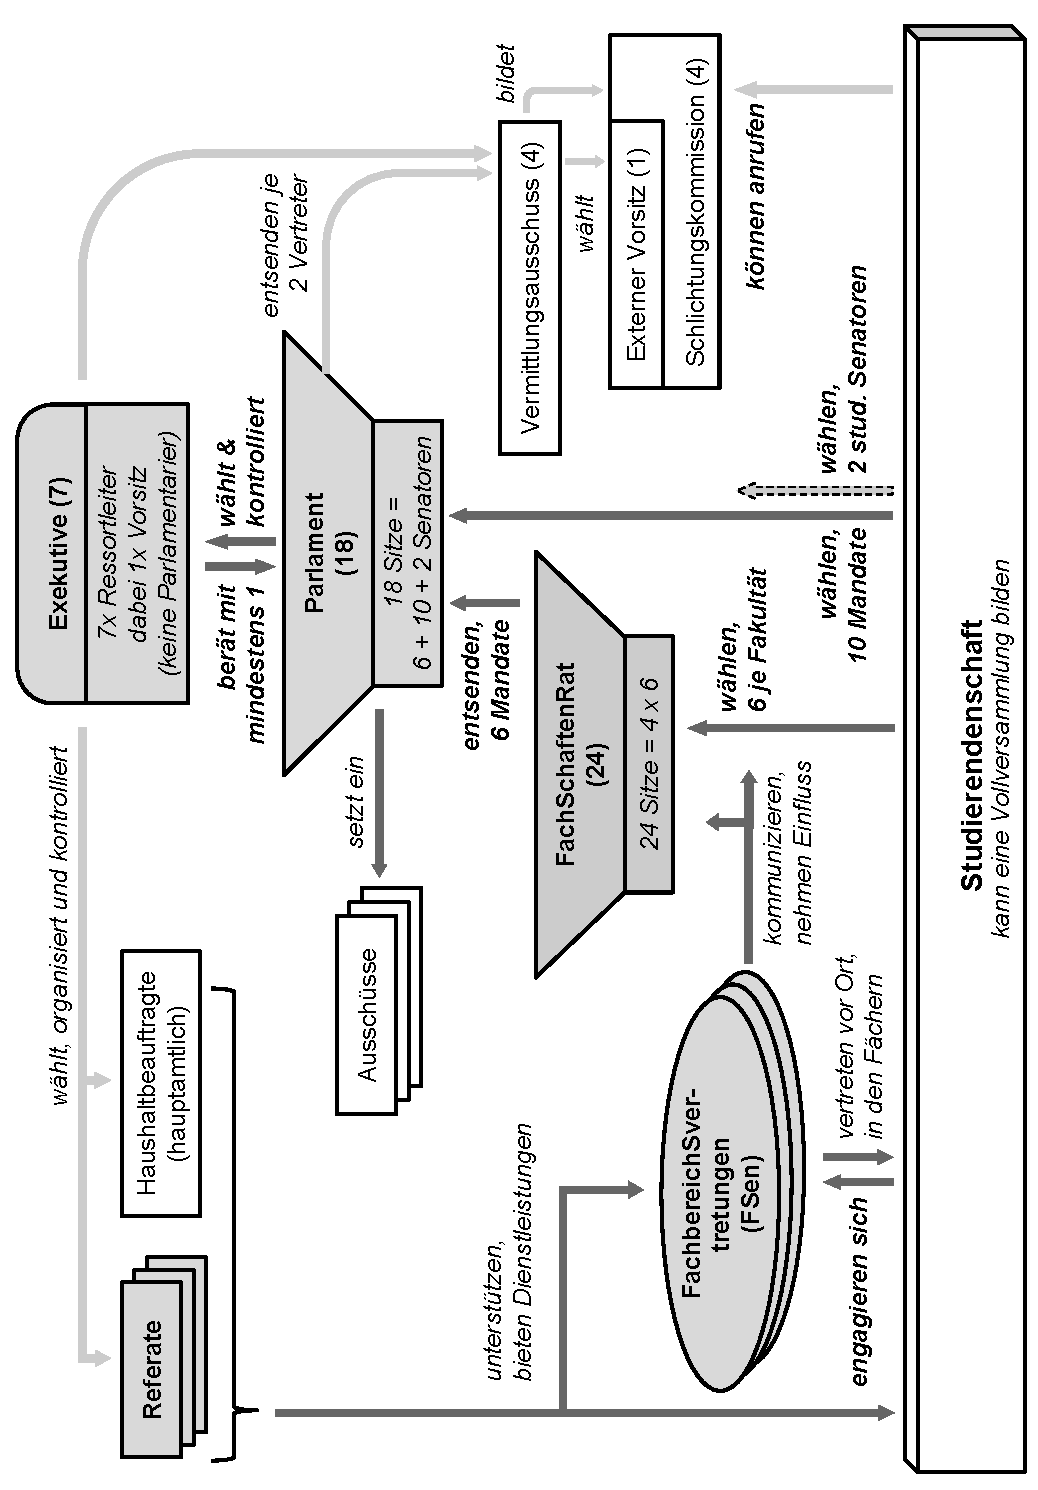
\includepdf
	[
		height = 0.9\paperheight,
		width = 0.8\paperwidth,
		keepaspectratio
	]
	{./teile/93-struktur-besetzung-kontrolle.pdf}



\backmatter

% !TeX root = ../stuve-handbuch-1.tex
% !TeX encoding = UTF-8
% !TeX spellcheck = de_DE
% !TeX program = pdflatex


\thispagestyle{empty}
\null\vfill
\begin{center}
	{\normalsize \textipa{/,ju:z3'bIlIti/}}
%	Freiraum!
\end{center}
\vfill\null\vfill
\clearpage

\thispagestyle{empty}
\null\vfill

\begin{center}
\begin{minipage}{0.7\textwidth}
%\scriptsize

Es gibt aktuell die folgenden \textbf{„StuVe-Handbücher“}

\textbf{\begin{enumerate}[\hspace{3em}1:]
	\item Gremien, Beschlüsse und Statuten
	\item Finanzen
	\item Veranstaltungsleitfaden
	\item Büro-ABC
\end{enumerate}}
\null

Alle sind im Wiki zu finden und dementsprechend gibt es dort immer den aktuellsten Stand: \url{https://wiki.asta.uni-ulm.de/asta/Handbuch}. Bisweilen wird – wie hier vorliegend – von manchen Handbüchern auch eine gedruckte Version erstellt.

\end{minipage}
\end{center}


\vfill\null\vfill
%\vspace{16.5cm}
\begin{center}
	
\includegraphics[keepaspectratio, width=5em]{./grafiken/stuve_logo_gedreht-leicht_grau.png}\\
	\textcolor{black!40}{\large \textbf{uuulm}}
\end{center}



\end{document}
